\chapter{Desenvolvimento}

Neste capítulo, apresento detalhadamente todas as etapas envolvidas no desenvolvimento da plataforma web para projeto, visualização gráfica e cálculo automatizado do orçamento óptico em redes \gls{pon}. A abordagem contempla desde o planejamento inicial até a consolidação da solução computacional. Inicialmente, estabeleço a especificação dos requisitos funcionais e não funcionais, bem como as restrições técnicas e operacionais que orientaram o projeto. Em seguida, descrevo o processo de prototipação da interface gráfica (\textit{wireframes}) e a definição da arquitetura de software adotada. Na sequência, detalho a modelagem de dados serializada em formato \gls{json}, os diagramas arquiteturais e os fluxos e algoritmos de cálculo de atenuação óptica codificados no \textit{backend}. Por fim, apresento a implementação prática da solução, detalhando a estrutura modular do código-fonte em FastAPI, a integração com a biblioteca gráfica D3.js no \textit{frontend} e o ambiente de conteinerização para implantação do sistema.

\section{Análise e Especificação de Requisitos}

Na etapa de análise e especificação de requisitos busquei mapear as necessidades operacionais de projetistas e engenheiros de redes \gls{ftth}/\gls{pon}, garantindo que o sistema ofereça precisão matemática nos cálculos de atenuação e facilidade de manipulação visual da topologia. A seguir, são detalhados os requisitos funcionais, os requisitos não funcionais e as restrições do sistema.

\subsection{Requisitos Funcionais}

Os Requisitos Funcionais descrevem as ações, cálculos e comportamentos que o sistema deve executar para atender às necessidades do usuário:

\begin{itemize}
    \item \textbf{Criação e Edição Interativa da Topologia:} O sistema deve permitir ao usuário construir e modificar visualmente a árvore da rede, inserindo, movendo e removendo elementos típicos de rede \gls{pon}, tais como \gls{olt}, caixas de emenda/fusão, \textit{splitters} (balanceados e desbalanceados), \gls{cto} e \gls{onu}.
    
    \item \textbf{Cálculo Automatizado do Orçamento Óptico:} O sistema deve calcular automaticamente a perda acumulada de potência ao longo de cada enlace, considerando a atenuação distribuída da fibra por quilômetro.
    
    \item \textbf{Contabilização de Atenuações Concentradas:} O sistema deve computar as perdas pontuais de inserção introduzidas por conectores ópticos, emendas/fusões de fibra e elementos passivos de divisão (\textit{splitters} balanceados e desbalanceados).
    
    \item \textbf{Validação por Classe de Transceptor:} O sistema deve parametrizar e validar os níveis de potência de transmissão ($T_x$) e os limites de sensibilidade do receptor ($R_x$) de acordo com as classes normatizadas.
    
    \item \textbf{Indicação do Status do Link:} O sistema deve sinalizar visualmente em tempo real se a potência óptica que atinge cada nó de terminação \gls{onu} está dentro dos limites operacionais adequados, exibindo alertas em caso de sinal degradado ou fora da margem de sensibilidade.
    
    \item \textbf{Persistência de Projetos em \gls{json}:} O sistema deve permitir salvar, carregar, atualizar e exportar a estrutura completa da topologia da rede e seus parâmetros de configuração em arquivos no formato \gls{json}.
    
    \item \textbf{Gerenciamento de Projetos e Pastas:} O sistema deve fornecer uma interface para organização de múltiplos arquivos de projeto dentro de diretórios no ambiente do servidor.
\end{itemize}

\subsection{Requisitos Não Funcionais}

Os Requisitos Não Funcionais definem os critérios de qualidade, desempenho, usabilidade e infraestrutura exigidos pela aplicação:

\begin{itemize}
    \item \textbf{Arquitetura em Camadas e Desacoplamento:} O \textit{backend} deve ser implementado em Python utilizando o \textit{framework} FastAPI, seguindo o padrão de projeto \gls{mvc} para separação clara entre rotas, regras de negócio e persistência.
    
    \item \textbf{Renderização Gráfica de Alto Desempenho:} A interface gráfica (\textit{frontend}) deve utilizar a biblioteca manipuladora de grafos D3.js no navegador, garantindo renderização fluida e reativa da estrutura da rede em tempo real.
    
    \item \textbf{Portabilidade e Conteinerização:} A aplicação deve fornecer suporte completo a contêineres Docker e orquestração via Docker Compose, permitindo execução simples e padronizada em ambientes de desenvolvimento e produção independente do sistema operacional hospedeiro.
    
    \item \textbf{Baixo Tempo de Resposta:} As chamadas à \gls{api} REST para recalculo do orçamento óptico devem responder em tempo inferior a 200 milissegundos.
    
\end{itemize}

\subsection{Restrições do Sistema}

O escopo do desenvolvimento esteve sujeito às seguintes restrições técnicas e operacionais:

\begin{itemize}
    \item O sistema opera focado no cálculo de potência unidirecional do canal de \textit{downstream}. Não calcula a potência no sentido \textit{upstream}
    
    \item A persistência local é realizada diretamente no sistema de arquivos em formato \gls{json}, abrindo mão de um banco de dados para simplificar a implantação.
    
    \item O motor de visualização limita-se à representação lógica da topologia em formato de grafo em árvore ponto-multi-ponto, sem integração georreferenciada.
\end{itemize}

\subsection{Prototipação da Interface (Wireframes)}

Antes do início da codificação da interface gráfica final, elaborei protótipos de interface (\textit{wireframes}). O objetivo dessa etapa foi organizar a arquitetura de informação e validar a usabilidade do operador antes da integração com a biblioteca gráfica D3.js e o motor de cálculo.

A interface foi concebida em três áreas funcionais integradas:
\begin{itemize}
    \item \textbf{Barra de Ferramentas Lateral (\textit{Toolbar}):} Disposta à esquerda, agrupando os atalhos para inserção dos elementos de rede (\gls{olt}, \textit{Splitters} balanceados e desbalanceados, \gls{onu} e Caixas de Anotação/Texto).
    
    \item \textbf{Área Central de Modelagem (\textit{Canvas}):} Espaço interativo principal onde a topologia gráfica é desenhada e manipulada via arrasto, renderizando os enlaces de fibra e caixas de atendimento.
    
    \item \textbf{Painel de Propriedades e Orçamento Óptico:} Coluna lateral à direita dedicada à edição dos parâmetros do nó selecionado e exibição em tempo real do nível de sinal calculado.
\end{itemize}

A Figura~\ref{fig:wireframe_interface} ilustra a concepção estrutural da interface do sistema.

\begin{figure}[htb]
    \caption{Esquema de \textit{wireframe} para a interface de modelagem gráfica}
    \centering
    \parbox{16cm}{
        \centering
        \label{fig:wireframe_interface}
        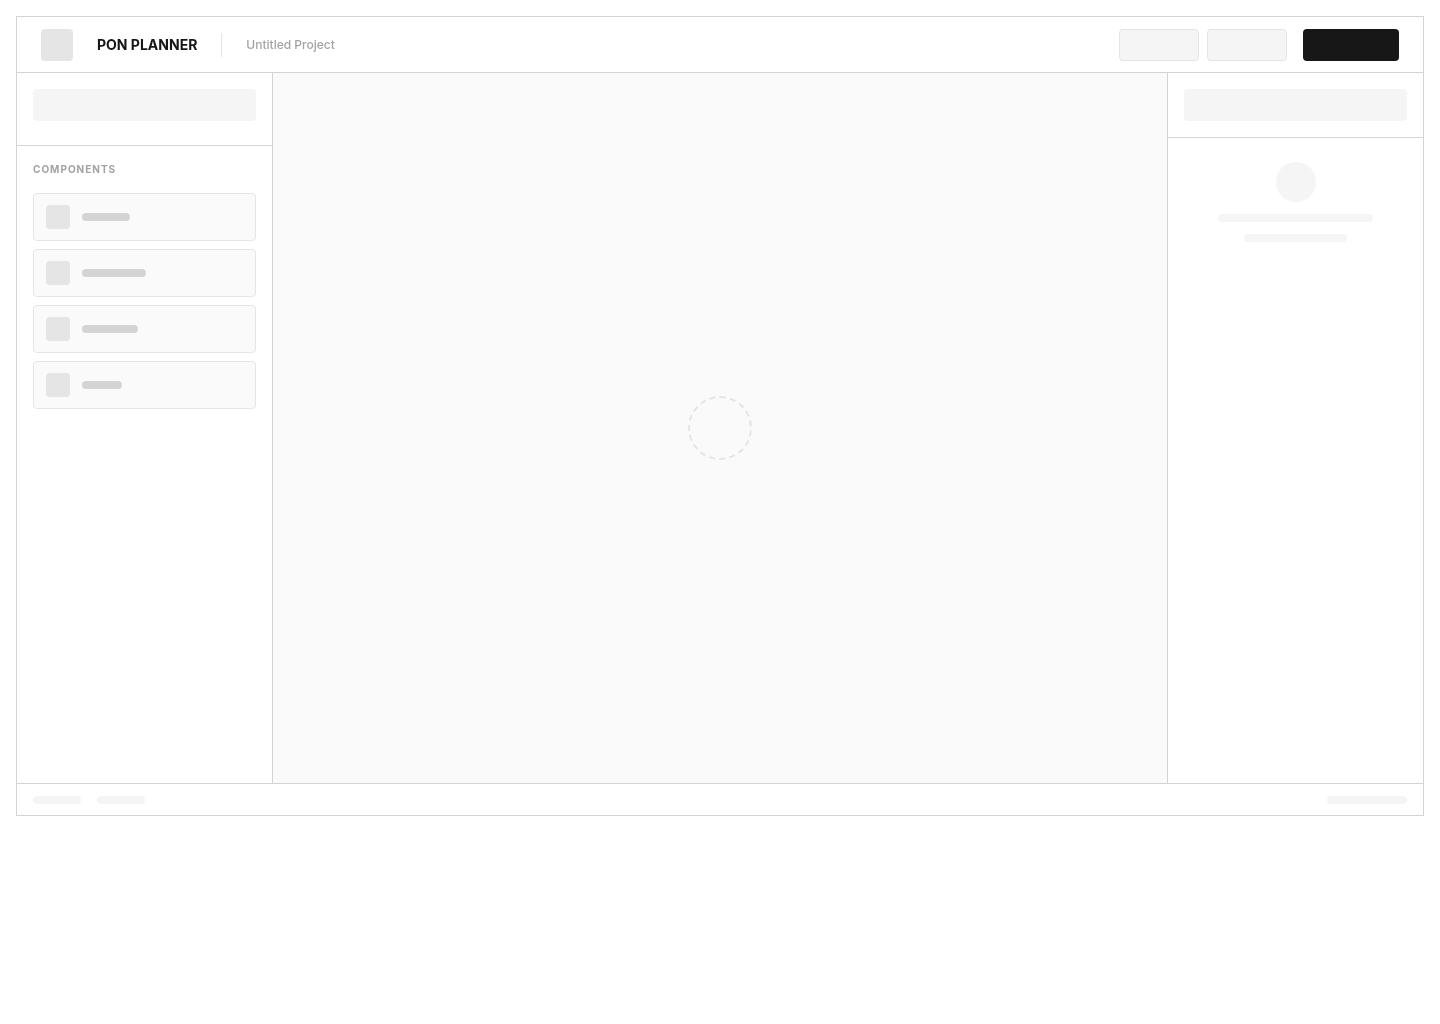
\includegraphics[width=\textwidth]{images/wireframe_interface.png}
        \par\footnotesize Fonte: Elaboração própria com auxílio de IA.
    }
\end{figure}

\section{Arquitetura do Sistema}

A arquitetura de software da plataforma foi desenvolvida com base no desacoplamento entre a camada de apresentação (\textit{frontend}) e a camada de serviços e regras de negócio (\textit{backend}). Essa abordagem garante modularidade, facilita a manutenção do código e permite que o cálculo do orçamento óptico seja consumido como um serviço independente por meio de uma \gls{api} RESTful. A seguir, detalho a visão geral da arquitetura, a organização de seus componentes internos e o modelo de implantação conteinerizado.

\subsection{Visão Geral da Arquitetura}

O sistema adota o padrão cliente-servidor para aplicações web de página única \gls{spa}. O \textit{frontend} é executado diretamente no navegador do usuário, sendo responsável por renderizar a interface gráfica e capturar interações da topologia. A comunicação com o \textit{backend} ocorre de forma assíncrona por meio de requisições \gls{http} enviando e recebendo dados estruturados em formato \gls{json}.

Na Figura~\ref{fig:arquitetura_geral}, apresento a visão geral da arquitetura do sistema e o fluxo de interação entre o usuário, o cliente web e o servidor de aplicação.

\begin{figure}[htb]
    \caption{Visão geral da arquitetura do sistema}
    \centering
    \parbox{16cm}{
        \centering
        \label{fig:arquitetura_geral}
        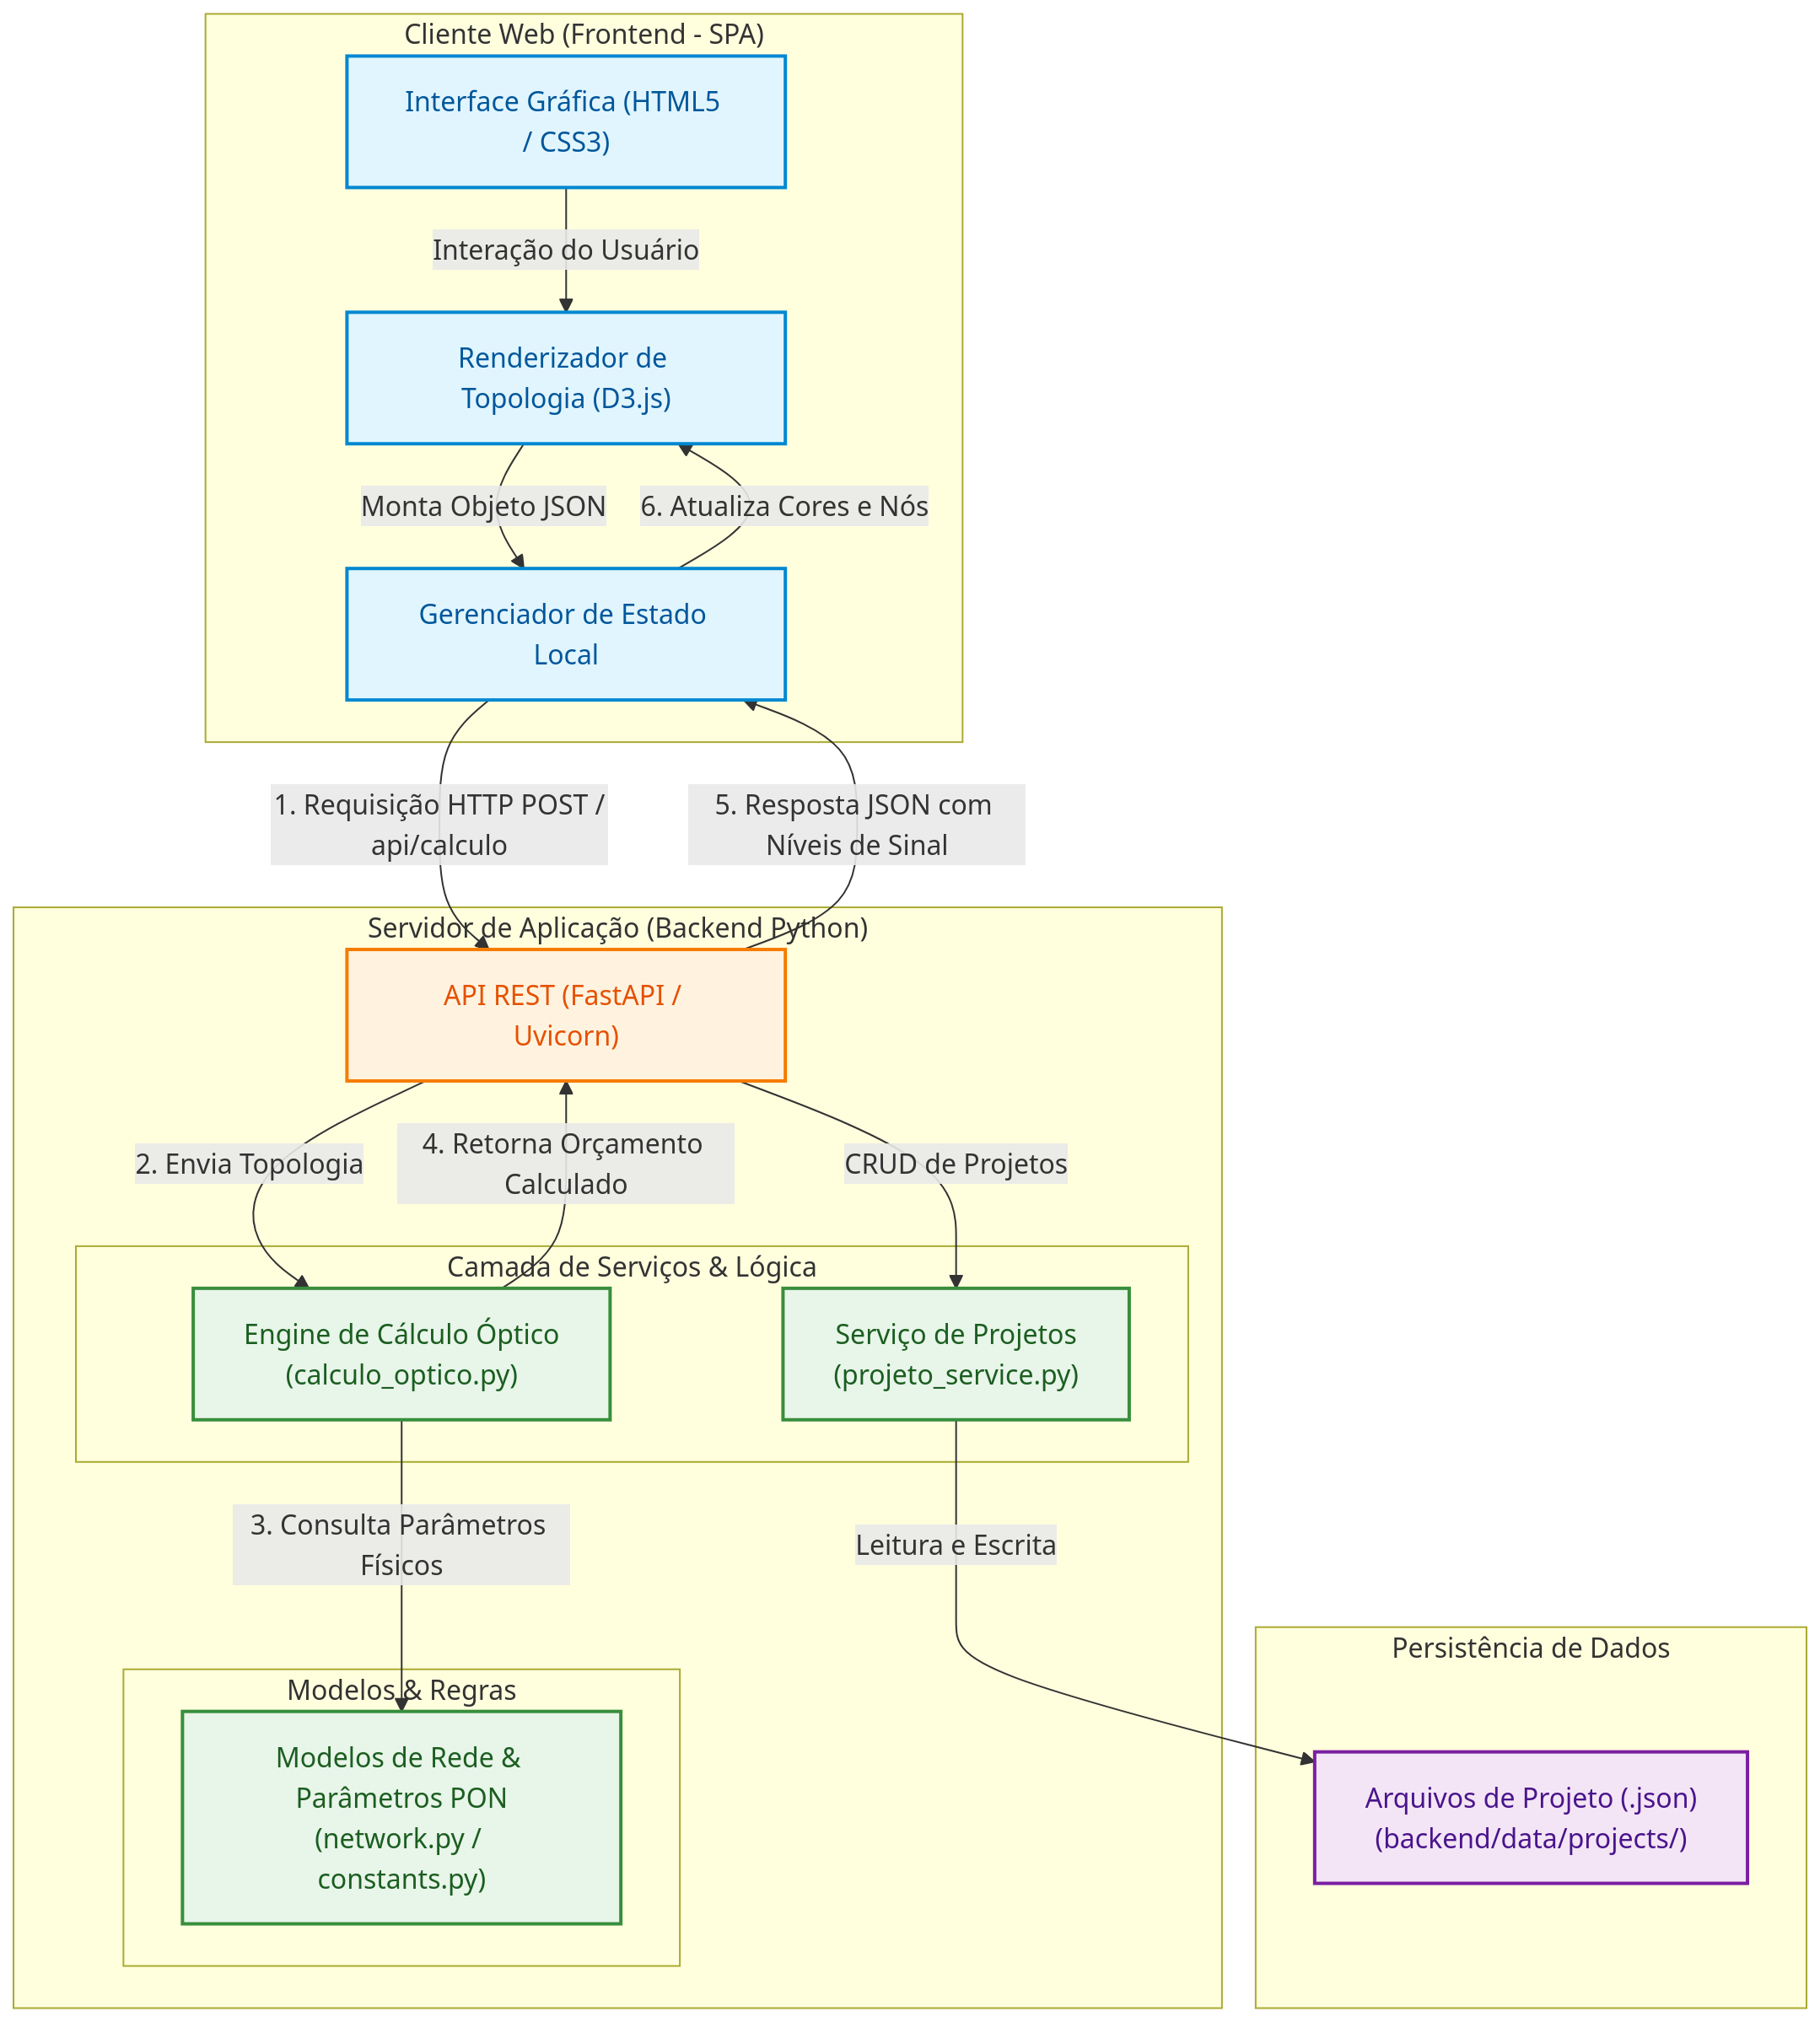
\includegraphics[width=\textwidth]{images/arquitetura_geral.png}
        \par\footnotesize Fonte: Elaboração própria com auxílio de IA.
    }
\end{figure}

Ao realizar qualquer alteração na topologia (como adicionar um nó ou alterar o comprimento de um trecho de fibra), o \textit{frontend} monta o objeto da rede em \gls{json} e o dispara para o \textit{endpoint} de cálculo do \textit{backend}. O servidor processa a topologia, efetua a soma das atenuações e retorna os níveis de sinal calculados para cada nó, permitindo a atualização imediata da interface visual.

\subsection{Diagrama de Componentes}

O \textit{backend} foi estruturado sob o padrão \gls{mvc}, utilizando o \textit{framework} FastAPI. A organização dos componentes é subdividida em três camadas principais:

\begin{itemize}
    \item \textbf{Controladores (\textit{Controllers}):} Módulos responsáveis por expor as rotas da \gls{api} REST e tratar as requisições \gls{http}. O controlador \texttt{calculo.py} recebe as estruturas de rede para validação e recalculo; o controlador \texttt{projetos.py} lida com operações de criação, leitura, atualização e exclusão de arquivos de topologia; e o controlador \texttt{pastas.py} gerencia a organização dos arquivos no servidor.
    
    \item \textbf{Serviços (\textit{Services}):} Concentram a lógica de negócio do sistema. O serviço \texttt{calculo\_optico.py} contém os algoritmos matemáticos que percorrem a árvore da rede e somam as perdas distribuídas e concentradas. O serviço \texttt{projeto\_service.py} gerencia o manuseio e a serialização de dados no sistema de arquivos.
    
    \item \textbf{Modelos e Constantes (\textit{Models}):} O arquivo \texttt{network.py} estabelece as estruturas de dados para representação de nós, conexões e redes. O arquivo \texttt{constants.py} armazena os parâmetros físicos normatizados, tais como coeficientes de atenuação de conectores, emendas, \textit{splitters}.
\end{itemize}

A Figura~\ref{fig:diagrama_componentes} ilustra o Diagrama de Componentes do sistema, detalhando a divisão modular interna e as dependências entre controladores, serviços e modelos.

\begin{figure}[htb]
    \caption{Diagrama de componentes do \textit{backend}}
    \centering
    \parbox{16cm}{
        \centering
        \label{fig:diagrama_componentes}
        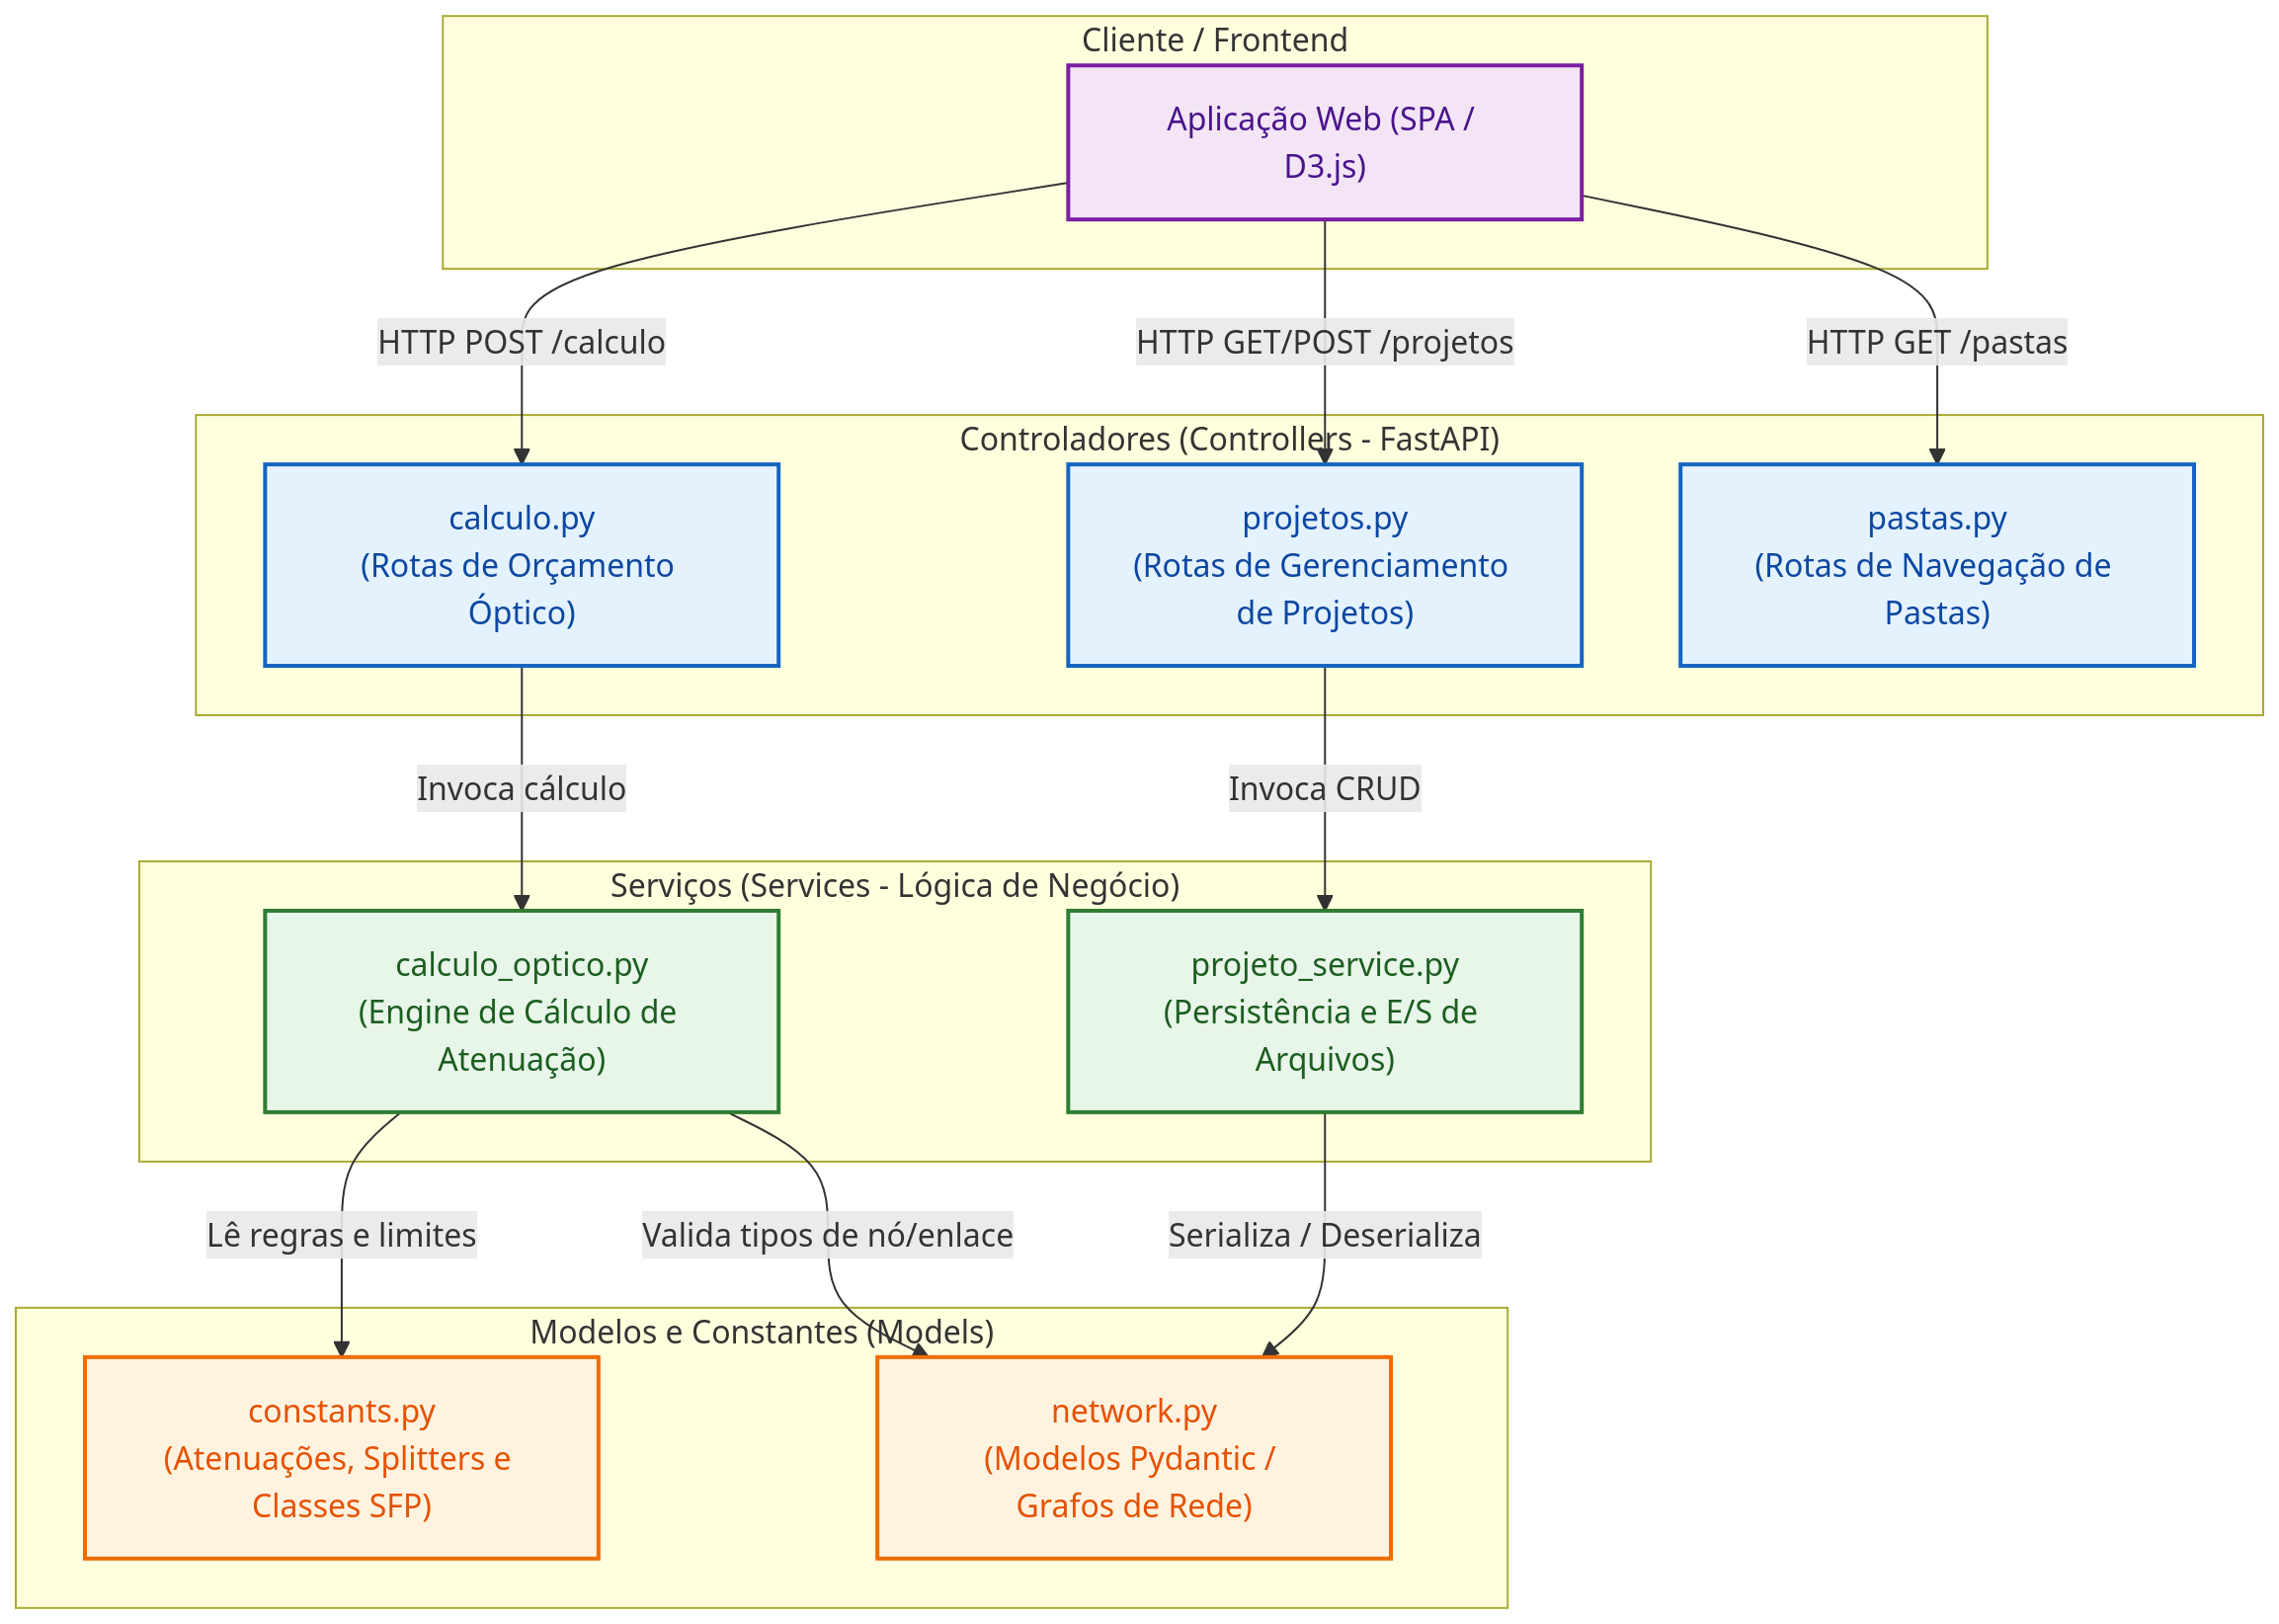
\includegraphics[width=\textwidth]{images/diagrama_componentes.png}
        \par\footnotesize Fonte: Elaboração própria com auxílio de IA.
    }
\end{figure}

\subsection{Diagrama de Implantação}

Para garantir a portabilidade e a facilidade de distribuição da plataforma, adotei a conteinerização da aplicação utilizando Docker. O ambiente é orquestrado por meio do Docker Compose, isolando a execução do servidor FastAPI e de suas dependências em um contêiner padronizado.

Na Figura~\ref{fig:diagrama_implantacao}, apresento o Diagrama de Implantação do sistema, destacando o ambiente de execução containerizado e a exposição da porta de atendimento de requisições.

\begin{figure}[htb]
    \caption{Diagrama de implantação do sistema containerizado}
    \centering
    \parbox{16cm}{
        \centering
        \label{fig:diagrama_implantacao}
        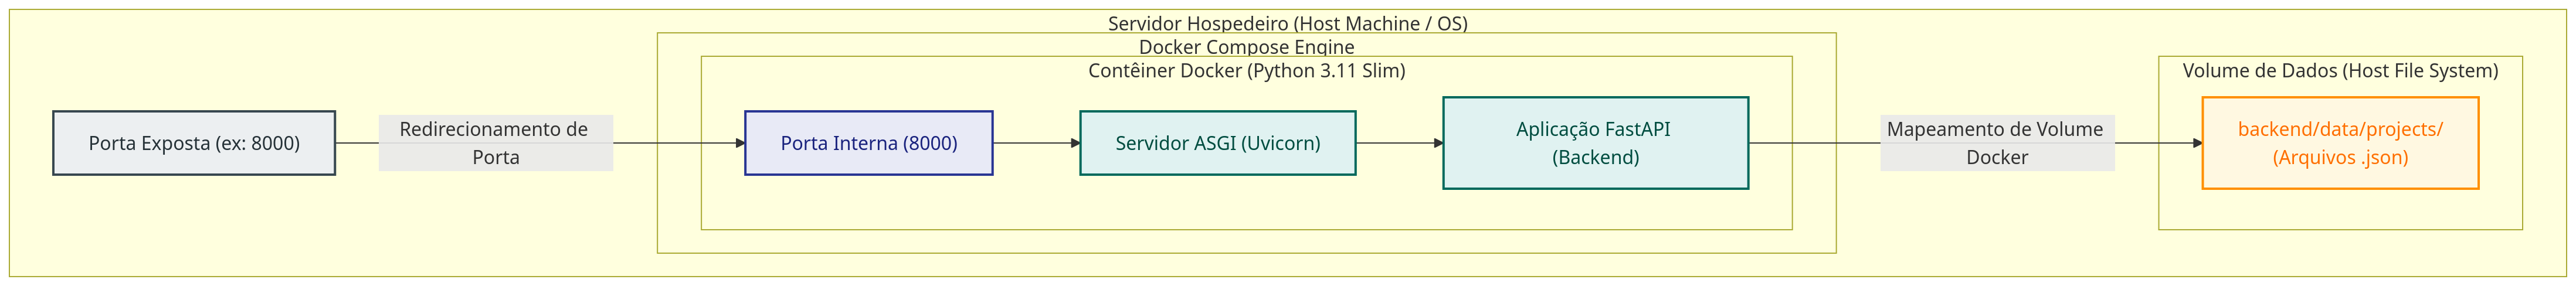
\includegraphics[width=\textwidth]{images/diagrama_implantacao.png}
        \par\footnotesize Fonte: Elaboração própria com auxílio de IA.
    }
\end{figure}

O arquivo \texttt{Dockerfile} especifica a imagem base Python, a instalação das dependências declaradas em \texttt{requirements.txt} e a inicialização do servidor de aplicação Uvicorn. O \texttt{docker-compose.yml} faz o mapeamento das portas do hospedeiro para o contêiner e configura os volumes de dados para garantir a persistência dos projetos salvos em formato \gls{json} no diretório \texttt{backend/data/projects}.

\section{Modelagem de Dados}
\label{sec:modelagem_dados}

Para a representação da topologia de rede óptica e persistência dos projetos, optei por uma estrutura de dados serializada em formato \gls{json}. Essa modelagem baseada em grafos confere leveza ao sistema e flexibilidade para a manipulação dos nós e enlaces tanto no \textit{frontend} quanto no \textit{backend}, eliminando a necessidade de um banco de dados relacional complexo. A seguir, detalho a estrutura conceitual e o esquema completo do documento de projeto.

\subsection{Modelo Conceitual e Estrutura dos Dados}

O projeto é representado por um documento \gls{json} autocontido composto por quatro blocos de dados essenciais:

\begin{itemize}
    \item \textbf{Metadados e Parâmetros Globais (\texttt{parametros}):} Define as configurações globais do projeto, incluindo atenuador padrão da fibra ($\text{dB/km}$), perda por conectorização, perda por fusão e margem de segurança do sistema em dB.
    
    \item \textbf{Nós da Rede (\texttt{nos}):} Conjunto de elementos que compõem a topologia. Cada nó possui atributos de identificação (\texttt{id}, \texttt{nome}), coordenadas de renderização espacial (\texttt{posicao}), e propriedades específicas de acordo com o seu tipo:
    \begin{itemize}
        \item \textit{\gls{olt}:} Armazena a potência de transmissão (\texttt{potencia\_tx\_dbm}), sensibilidade de recepção (\texttt{sensibilidade\_rx\_dbm}) e o padrão de rede (\texttt{padrao\_pon}).
        \item \textit{Splitter:} Suporta divisões balanceadas e desbalanceadas, registrando a razão de divisão (\texttt{razao}), a indicação do tipo (\texttt{tipo\_splitter}) e a fração desbalanceada (\texttt{razao\_desbalanceada}, ex.: 10/90, 20/80).
        \item \textit{\gls{onu}:} Ponto terminal de atendimento que especifica a sensibilidade óptica mínima exigida (\texttt{sensibilidade\_rx\_dbm}).
        \item \textit{Texto:} Elemento visual utilitário utilizado para delimitação gráfica e identificação das caixas de atendimento na interface (ex.: Caixas de Emenda, CTOs 377, 378, 379).
    \end{itemize}
    
    \item \textbf{Enlaces e Conexões (\texttt{enlaces}):} Mapeia as conexões direcionadas entre um nó de origem (\texttt{id\_origem}) e um nó de destino (\texttt{id\_destino}). Cada enlace armazena o comprimento do trecho em metros (\texttt{comprimento\_m}), a taxa de atenuação específica, o número de conexões/fusões, e a atenuação individual introduzida pelas portas dos \textit{splitters} (\texttt{perda\_splitter\_db}).
\end{itemize}

\subsection{Esquema do Arquivo JSON de Projeto}

Abaixo, apresento a estrutura de um arquivo de projeto serializado implementado no sistema, exemplificando a integração dos nós, enlaces e parâmetros globais de cálculo:

\begin{verbatim}
{
  "id": "projeto-yol156nu",
  "nome": "pon-5-1",
  "parametros": {
    "atenuacao_fibra_db_por_km": 0.35,
    "perda_conector_db": 0.5,
    "perda_fusao_db": 0.03,
    "margem_sistema_db": 3
  },
  "nos": [
    {
      "id": "olt-1",
      "tipo": "OLT",
      "nome": "pon 5/1",
      "potencia_tx_dbm": 5.0,
      "sensibilidade_rx_dbm": -28.0,
      "padrao_pon": "GPON",
      "posicao": { "x": -369.0, "y": 260.0 }
    },
    {
      "id": "splitter-2",
      "tipo": "Splitter",
      "nome": "10/90",
      "razao": 8,
      "tipo_splitter": "desbalanceado",
      "razao_desbalanceada": "10/90",
      "posicao": { "x": 230.0, "y": 256.0 }
    },
    {
      "id": "onu-3",
      "tipo": "ONU",
      "nome": "SINAL 1x8",
      "sensibilidade_rx_dbm": -27.0,
      "posicao": { "x": 262.0, "y": -43.0 }
    }
  ],
  "enlaces": [
    {
      "id": "lnk-3",
      "id_origem": "splitter-1",
      "id_destino": "splitter-2",
      "comprimento_m": 100.0,
      "atenuacao_db_por_km": 0.35,
      "tipo_conexao": "fusao",
      "num_conexoes": 2,
      "perda_por_conexao_db": 0.03,
      "perda_splitter_db": 0.36
    }
  ]
}
\end{verbatim}

Essa estrutura permite que todo o cálculo do orçamento óptico seja realizado de forma iterativa percorrendo os \textit{arrays} \texttt{nos} e \texttt{enlaces}, garantindo que atualizações de topologia sejam sincronizadas de forma ágil entre a interface visual e o motor de cálculo.

\section{Modelagem de Processos}

Nesta seção, apresento o funcionamento lógico da aplicação e o algoritmo responsável pelo processamento e cálculo do orçamento óptico ao longo da topologia de rede. A modelagem de processos descreve o fluxo de dados desde a captura das interações na interface gráfica até a execução dos cálculos matemáticos de atenuação no \textit{backend}.

\subsection{Fluxo Principal de Sinalização e Cálculo}

O fluxo de processamento é disparado de forma reativa a cada modificação realizada pelo usuário na interface gráfica. A interação segue um modelo assíncrono cliente-servidor, garantindo que o cálculo do orçamento de potência seja processado e refletido visualmente em milissegundos.

A Figura~\ref{fig:fluxo_calculo} ilustra o Diagrama de Sequência que detalha a sinalização e o fluxo de dados entre o usuário, a interface em D3.js, o controlador da \gls{api} e o motor de cálculo do \textit{backend}.

\begin{figure}[htb]
    \caption{Fluxo de sinalização e cálculo do orçamento óptico}
    \centering
    \parbox{16cm}{
        \centering
        \label{fig:fluxo_calculo}
        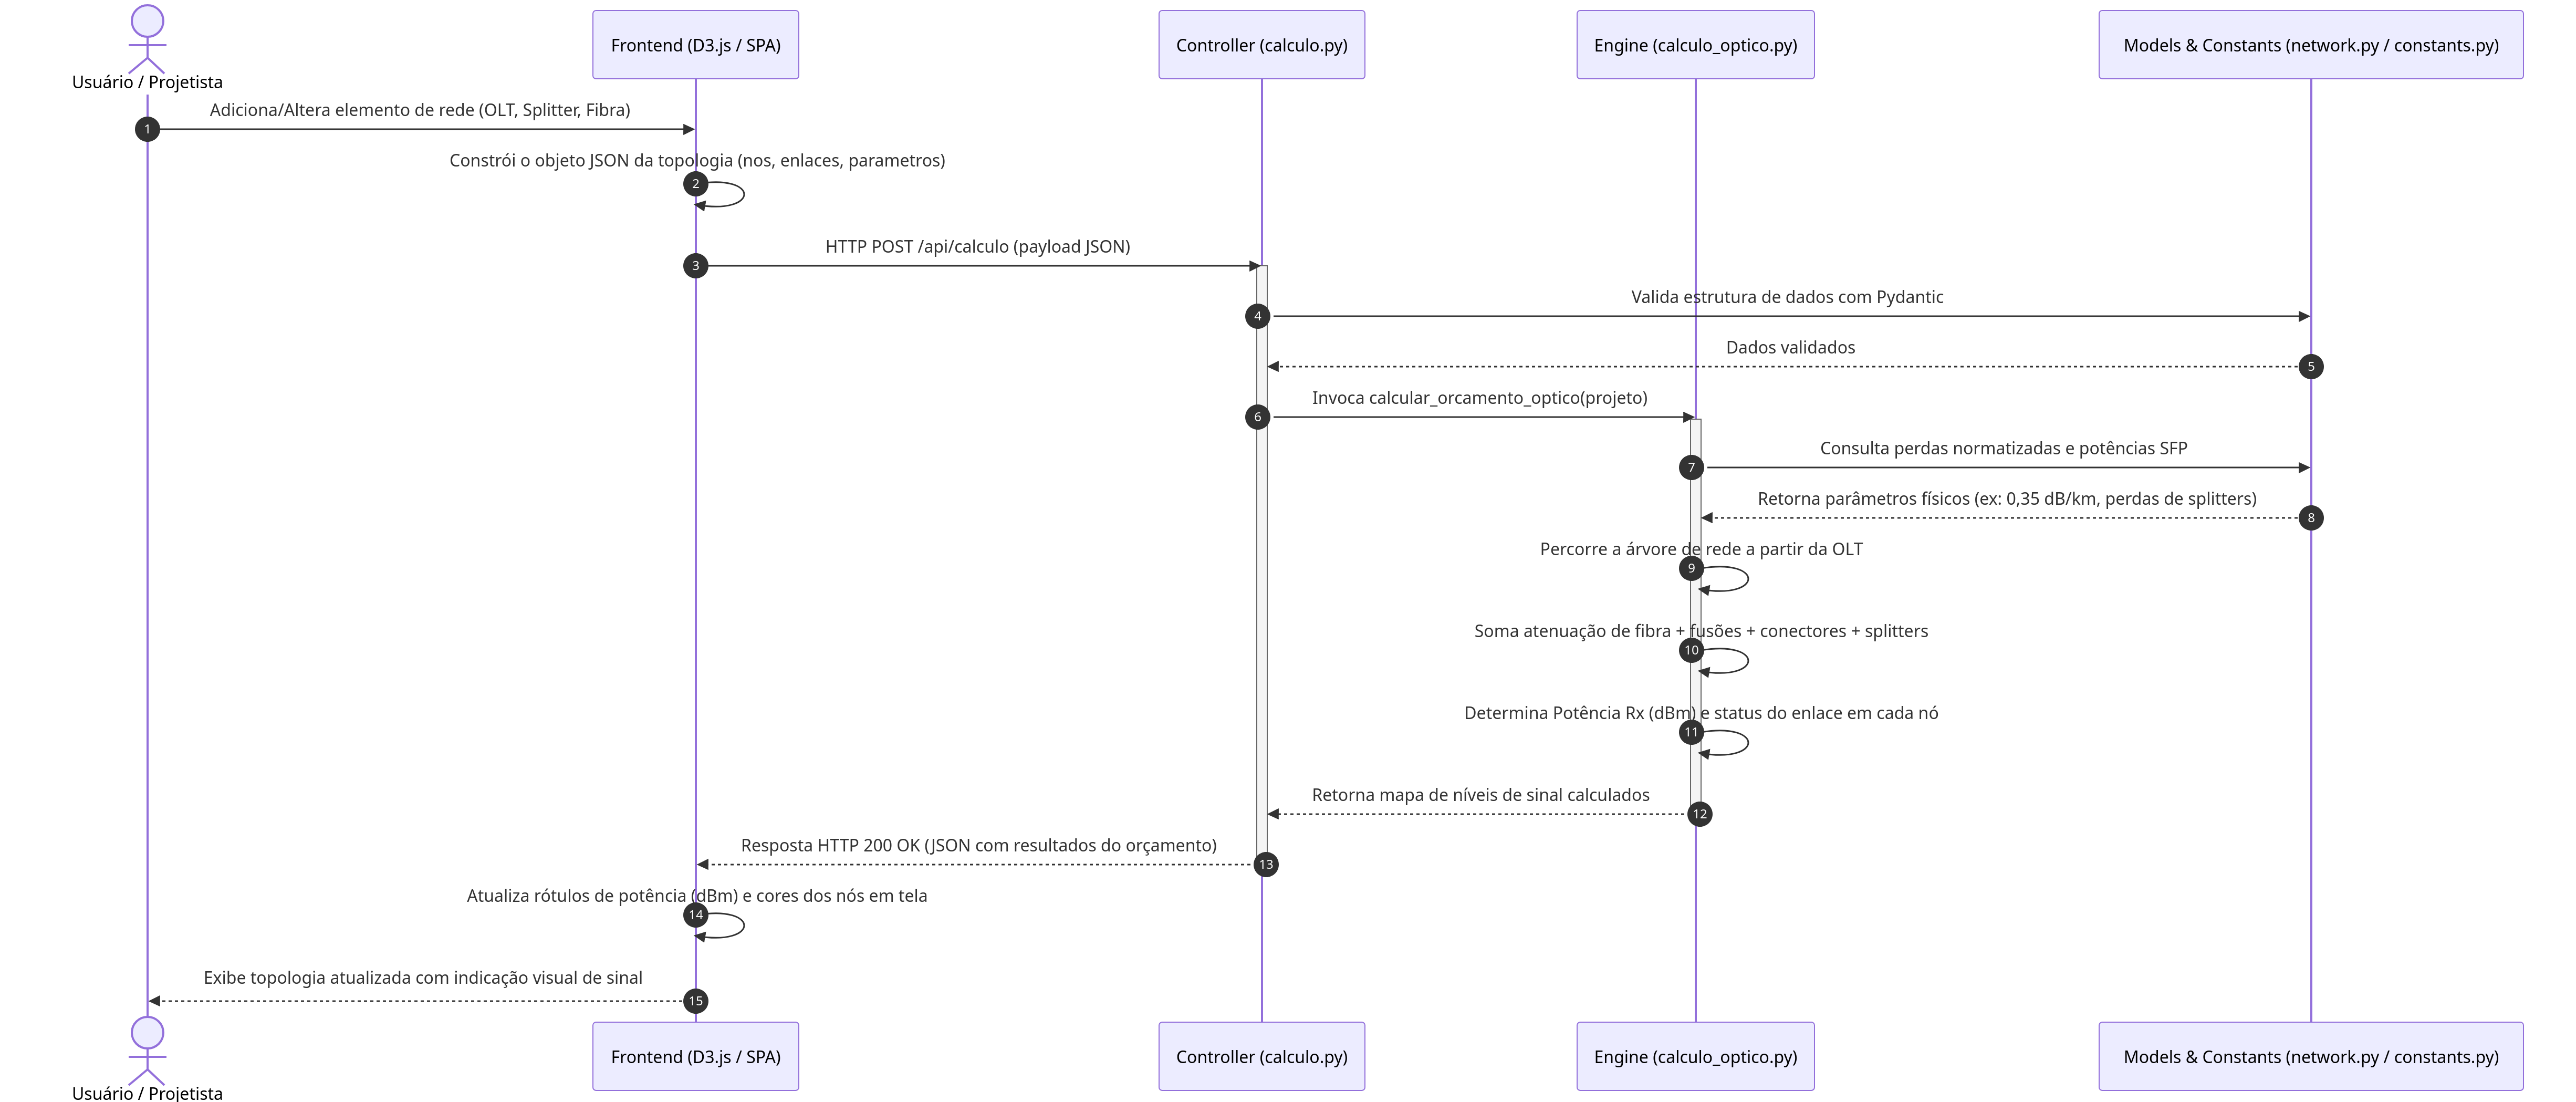
\includegraphics[width=\textwidth]{images/fluxo_calculo.png}
        \par\footnotesize Fonte: Elaboração própria com auxílio de IA.
    }
\end{figure}

O ciclo de execução ilustrado compreende as seguintes etapas encadeadas:

\begin{enumerate}
    \item \textbf{Captura da Ação:} O usuário altera a topologia (ex.: altera a distância de um cabo de fibra óptica ou altera a razão de um \textit{splitter}).
    \item \textbf{Serialização:} O \textit{frontend} lê a estrutura do grafo manipulado via D3.js e monta o documento \gls{json} padronizado com os nós, enlaces e parâmetros de rede.
    \item \textbf{Requisição HTTP:} A aplicação envia uma requisição \gls{http} \texttt{POST} assíncrona contendo o estado da rede para a rota \texttt{/api/calculo}.
    \item \textbf{Validação e Processamento:} O controlador valida os dados via Pydantic e aciona o motor de cálculo em Python (\texttt{calculo\_optico.py}), que percorre iterativamente a árvore da rede somando as perdas do trecho.
    \item \textbf{Renderização Visual:} O \textit{backend} retorna a lista de nós com seus respectivos valores de potência estimada. O \textit{frontend} atualiza imediatamente os rótulos de sinal em tela e aplica códigos de cores (verde para sinal dentro da margem, amarelo para atenção e vermelho para degradação/inoperância).
\end{enumerate}

\subsection{Algoritmo de Cálculo do Orçamento Óptico}

A lógica matemática de atenuação implementada em \texttt{calculo\_optico.py} calcula a perda acumulada ($A_{\text{total}}$) de cada caminho óptico até as terminações (\gls{onu}/\gls{cto}). A atenuação total de um enlace é dada pela soma das perdas distribuídas e concentradas, conforme a Equação:

\begin{equation}
A_{\text{total}} = (\alpha_{\text{fibra}} \cdot d) + (N_{\text{fusao}} \cdot \alpha_{\text{fusao}}) + (N_{\text{con}} \cdot \alpha_{\text{con}}) + \alpha_{\text{splitter}}
\end{equation}

Em que:
\begin{itemize}
    \item $\alpha_{\text{fibra}}$ é o coeficiente de atenuação da fibra óptica em dB/km (definido tipicamente em 0,35~dB/km);
    \item $d$ é a distância total do trecho em quilômetros;
    \item $N_{\text{fusao}}$ e $\alpha_{\text{fusao}}$ representam a quantidade de fusões/emendas e a atenuação por fusão (0,1~dB por padrão), respectivamente;
    \item $N_{\text{con}}$ e $\alpha_{\text{con}}$ representam a quantidade de conectores e a atenuação por conectorização (0,3~dB para conectores SC/APC por padrão), respectivamente;
    \item $\alpha_{\text{splitter}}$ é a perda de inserção concentrada introduzida pelos \textit{splitters} presentes no trajeto (por exemplo, $\approx 10,5$~dB para \textit{splitters} 1:8 balanceados).
\end{itemize}

Com a atenuação acumulada calculada, o nível de potência óptica incidente na \gls{onu} ($P_{\text{rx}}$) é obtido subtraindo $A_{\text{total}}$ da potência de saída do emissor da \gls{olt} ($P_{\text{tx}}$):

\begin{equation}
P_{\text{rx}} = P_{\text{tx}} - A_{\text{total}}
\end{equation}

O resultado $P_{\text{rx}}$ é comparado com os limites de sensibilidade da \gls{onu}, permitindo classificar o sinal do nó como adequado, crítico ou inoperante.

\section{Implementação dos Módulos Técnicos do Backend}
\label{sec:modulos_backend}

Nesta seção, detalho a implementação dos módulos do \textit{backend} da aplicação. O servidor foi construído em Python 3.11 utilizando o \textit{framework} FastAPI, escolhido pelo alto desempenho, suporte nativo a operações assíncronas (\textit{async/await}) e validação automática de tipos com Pydantic.

\subsection{Estrutura de Diretórios e Módulos do \textit{Backend}}

A organização física dos arquivos no repositório separa claramente as responsabilidades da aplicação entre controladores \gls{rest}, lógica de negócio e modelos de dados:

\begin{verbatim}
TCC-Redes-PON-main/
├── docker-compose.yml        # Orquestração do container (raiz do projeto)
└── backend/
    ├── Dockerfile            # Imagem de execução do backend
    ├── main.py               # Ponto de entrada do servidor FastAPI
    ├── requirements.txt      # Dependências (FastAPI, Uvicorn, Pydantic)
    ├── app/
    │   ├── controllers/      # Controladores REST (calculo.py, projetos.py)
    │   ├── services/         # Regras de negócio (calculo_optico.py, projeto_service.py)
    │   └── models/           # Esquemas Pydantic e constantes (network.py)
    ├── data/projects/        # Repositório de arquivos JSON salvos
    └── tests/                # Suíte de testes automatizados com Pytest
\end{verbatim}

\subsection{Modelagem Pydantic e Esquema de Dados (\texttt{network.py})}

A validação dos dados no servidor é feita pela biblioteca Pydantic. As estruturas foram divididas em classes específicas para garantir a tipagem correta de cada componente.

O primeiro trecho define os parâmetros globais da rede e a posição cartesiana dos nós:

\begin{verbatim}
from pydantic import BaseModel
from typing import List, Optional

class ParametrosGlobais(BaseModel):
    atenuacao_fibra_db_por_km: float = 0.35
    perda_conector_db: float = 0.5
    perda_fusao_db: float = 0.03
    margem_sistema_db: float = 3.0

class Posicao(BaseModel):
    x: float
    y: float
\end{verbatim}

A classe \texttt{ParametrosGlobais} estabelece as taxas teóricas e coeficientes de atenuação padrão utilizados na ausência de especificações nos enlaces. Já a classe \texttt{Posicao} armazena a localização espacial $(x,y)$ utilizada no \textit{canvas} gráfico.

Em seguida, o esquema detalha os atributos dos nós e conexões de fibra:

\begin{verbatim}
class NoSchema(BaseModel):
    id: str
    tipo: str  # "OLT", "Splitter", "ONU", "Texto"
    nome: str
    posicao: Posicao
    potencia_tx_dbm: Optional[float] = None
    sensibilidade_rx_dbm: Optional[float] = None
    padrao_pon: Optional[str] = None
    razao: Optional[int] = None
    tipo_splitter: Optional[str] = None  # "balanceado" ou "desbalanceado"
    razao_desbalanceada: Optional[str] = None

class EnlaceSchema(BaseModel):
    id: str
    id_origem: str
    id_destino: str
    comprimento_m: float
    atenuacao_db_por_km: float = 0.35
    tipo_conexao: str = "fusao"
    num_conexoes: int = 2
    perda_por_conexao_db: float = 0.03

class ProjetoSchema(BaseModel):
    id: str
    nome: str
    parametros: ParametrosGlobais
    nos: List[NoSchema]
    enlaces: List[EnlaceSchema]
\end{verbatim}

O \texttt{NoSchema} utiliza campos opcionais para suportar diferentes equipamentos. Por exemplo, atributos como \texttt{potencia\_tx\_dbm} são exclusivos da OLT, enquanto \texttt{razao\_desbalanceada} aplica-se apenas a \textit{splitters} ópticos. O \texttt{ProjetoSchema} consolida o documento JSON completo.

\subsection{Camada de Serviços e Algoritmo de Cálculo Óptico (\texttt{calculo\_optico.py})}

O arquivo \texttt{app/services/calculo\_optico.py} é o núcleo de cálculo do sistema. Ele interpreta a topologia como um grafo e calcula iterativamente a atenuação do sinal a partir da OLT.

A Figura~\ref{fig:fluxo_percurso_grafo} ilustra o fluxo sequencial do algoritmo de travessia do grafo e cálculo de atenuação acumulada.

\begin{figure}[htb]
    \caption{Fluxograma do algoritmo de travessia do grafo e cálculo óptico}
    \centering
    \parbox{16cm}{
        \centering
        \label{fig:fluxo_percurso_grafo}
        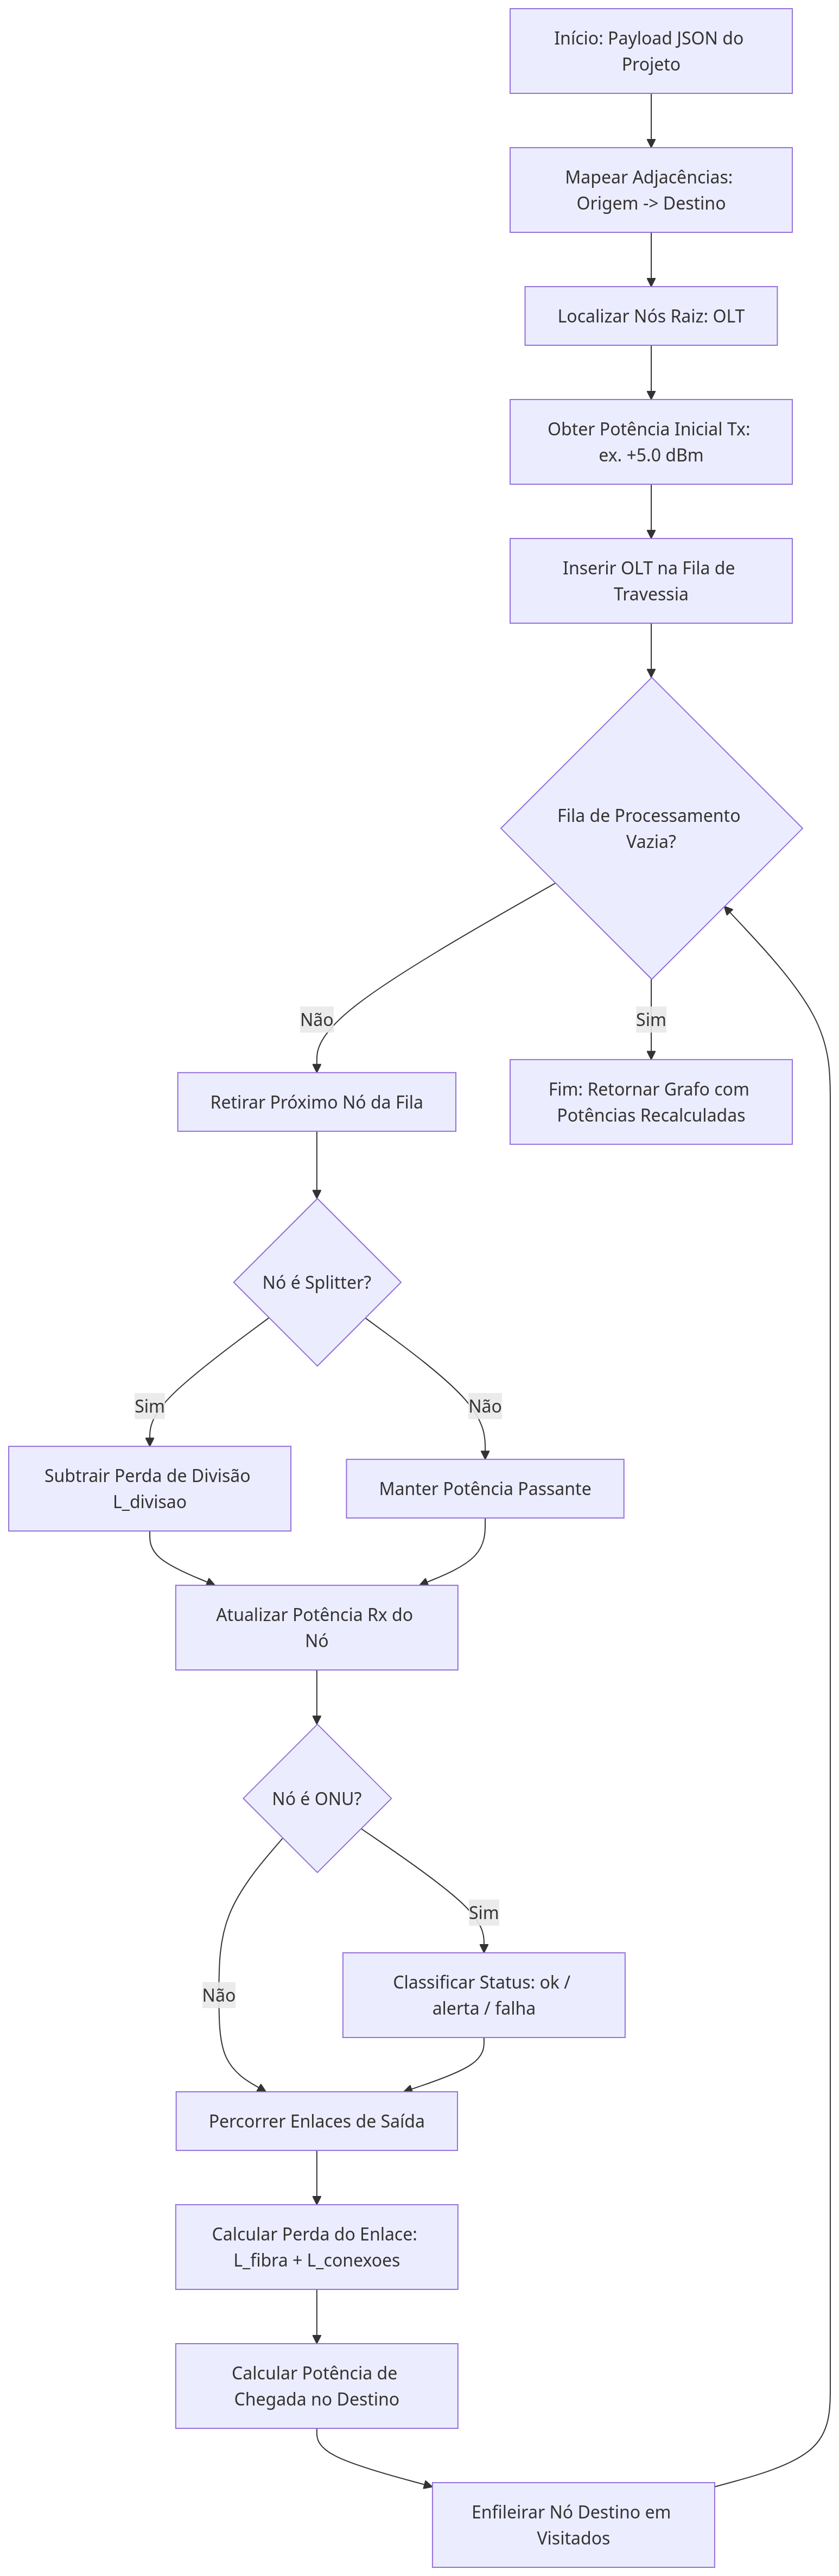
\includegraphics[width=0.35\textwidth]{images/fluxo_percurso_grafo.png}
        \par\footnotesize Fonte: Elaboração própria com auxílio de IA.
    }
\end{figure}

A implementação do motor de cálculo é dividida em três fases principais. A primeira fase realiza a montagem do mapa de adjacências e localiza o nó raiz:

\begin{verbatim}
import math
from typing import Dict, Any, List
from app.models.network import ProjetoSchema
from app.models.constants import PERDAS_SPLITTER_BALANCEADO, PERDAS_SPLITTER_DESBALANCEADO

def calcular_orcamento_optico(projeto: ProjetoSchema) -> Dict[str, Any]:
    nos_dict = {no.id: no.dict() for no in projeto.nos}
    
    # Mapeia as conexões de saída: id_origem -> lista de (enlace, id_destino)
    adjacencias: Dict[str, List[tuple]] = {no.id: [] for no in projeto.nos}
    for enlace in projeto.enlaces:
        if enlace.id_origem in adjacencias:
            adjacencias[enlace.id_origem].append((enlace, enlace.id_destino))

    # Identifica o nó emissor (OLT)
    olt = next((no for no in projeto.nos if no.tipo == "OLT"), None)
    if not olt:
        raise ValueError("A topologia não possui uma OLT cadastrada como raiz.")

    potencia_inicial = olt.potencia_tx_dbm if olt.potencia_tx_dbm is not None else 5.0
    nos_dict[olt.id]["potencia_rx"] = potencia_inicial
    nos_dict[olt.id]["status_sinal"] = "ok"
\end{verbatim}

Esta etapa converte a lista de enlaces em um dicionário de adjacências otimizado, permitindo que o algoritmo consulte as ramificações de saída de qualquer nó.

A segunda fase executa a travessia da rede utilizando uma fila de processamento:

\begin{verbatim}
    fila = [(olt.id, potencia_inicial)]
    visitados = set()

    while fila:
        no_atual_id, potencia_atual = fila.pop(0)
        visitados.add(no_atual_id)
        no_atual = nos_dict[no_atual_id]

        # Desconta a perda interna caso o nó seja um Splitter
        perda_interna_no = 0.0
        if no_atual["tipo"] == "Splitter":
            perda_interna_no = obter_perda_splitter(no_atual)

        potencia_apos_no = potencia_atual - perda_interna_no
        no_atual["potencia_rx"] = round(potencia_apos_no, 2)

        # Classifica o estado do sinal se o nó for uma ONU
        if no_atual["tipo"] == "ONU":
            sensibilidade = no_atual.get("sensibilidade_rx_dbm") or -27.0
            if potencia_apos_no >= sensibilidade:
                no_atual["status_sinal"] = "ok"
            elif potencia_apos_no >= (sensibilidade + projeto.parametros.margem_sistema_db):
                no_atual["status_sinal"] = "alerta"
            else:
                no_atual["status_sinal"] = "falha"
\end{verbatim}

Durante o laço, a atenuação do nó é subtraída do sinal incidente. Caso o nó seja uma ONU, o valor final $P_{\text{rx}}$ é comparado com o limiar de sensibilidade, atribuindo o estado funcional (\texttt{ok}, \texttt{alerta} ou \texttt{falha}).

A terceira fase estende a propagação do sinal ao longo dos enlaces conectados:

\begin{verbatim}
        # Propaga o sinal para os nós sucessores através dos enlaces de fibra
        for enlace, id_destino in adjacencias.get(no_atual_id, []):
            distancia_km = enlace.comprimento_m / 1000.0
            perda_fibra = distancia_km * enlace.atenuacao_db_por_km
            perda_conexoes = enlace.num_conexoes * enlace.perda_por_conexao_db
            
            perda_total_enlace = perda_fibra + perda_conexoes
            potencia_destino = potencia_apos_no - perda_total_enlace

            if id_destino not in visitados:
                fila.append((id_destino, potencia_destino))

    return {
        "nos": list(nos_dict.values()),
        "enlaces": [e.dict() for e in projeto.enlaces]
    }
\end{verbatim}

Para cada enlace, o código calcula a atenuação por quilometragem somada às perdas de acoplamentos mecânicos ou fusões. O resultado atualizado da potência é enfileirado para o próximo nó destino.

A função auxiliar para o cálculo de perda em \textit{splitters} é detalhada a seguir:

\begin{verbatim}
def obter_perda_splitter(no: dict) -> float:
    tipo = no.get("tipo_splitter", "balanceado")
    if tipo == "balanceado":
        razao = no.get("razao", 8)
        return PERDAS_SPLITTER_BALANCEADO.get(razao, 10.0 * math.log10(razao) + 0.5)
    elif tipo == "desbalanceado":
        razao_str = no.get("razao_desbalanceada", "10/90")
        return PERDAS_SPLITTER_DESBALANCEADO.get(razao_str, {}).get("passagem", 1.5)
    return 0.0
\end{verbatim}

\subsection{Serviços de Controladores e Persistência de Dados}

O controlador \gls{rest} \texttt{app/controllers/calculo.py} atua como intermediário entre a Web e a camada de serviço:

\begin{verbatim}
from fastapi import APIRouter, HTTPException, status
from app.models.network import ProjetoSchema
from app.services.calculo_optico import calcular_orcamento_optico

router = APIRouter(prefix="/api/calculo", tags=["Cálculo Óptico"])

@router.post("", status_code=status.HTTP_200_OK)
async def processar_calculo(projeto: ProjetoSchema):
    try:
        resultado = calcular_orcamento_optico(projeto)
        return {"status": "sucesso", "dados": resultado}
    except Exception as exc:
        raise HTTPException(
            status_code=status.HTTP_400_BAD_REQUEST,
            detail=f"Erro ao processar cálculo óptico: {str(exc)}"
        )
\end{verbatim}

Já a persistência dos arquivos \gls{json} no disco é realizada pelo serviço \texttt{ProjetoService} (\texttt{app/services/projeto\_service.py}):

\begin{verbatim}
import os
import json
from typing import List, Optional
from app.models.network import ProjetoSchema

CAMINHO_PROJETOS = os.path.join(os.path.dirname(__file__), "../../data/projects")

class ProjetoService:
    def __init__(self):
        os.makedirs(CAMINHO_PROJETOS, exist_ok=True)

    def obter_por_id(self, projeto_id: str) -> Optional[dict]:
        caminho = os.path.join(CAMINHO_PROJETOS, f"{projeto_id}.json")
        if not os.path.exists(caminho):
            return None
        with open(caminho, "r", encoding="utf-8") as f:
            return json.load(f)

    def salvar(self, projeto: ProjetoSchema) -> dict:
        caminho = os.path.join(CAMINHO_PROJETOS, f"{projeto.id}.json")
        with open(caminho, "w", encoding="utf-8") as f:
            json.dump(projeto.dict(), f, indent=4, ensure_ascii=False)
        return {"status": "sucesso", "id": projeto.id}
\end{verbatim}


\section{Implementação da Interface do Usuário (\textit{frontend})}

Nesta seção, apresento a implementação da interface gráfica do usuário. O \textit{frontend} foi construído sob o conceito de \gls{spa} centralizado no diretório \texttt{frontend/public/index.html}, utilizando a biblioteca D3.js (v7) para renderizaçao vetorial \gls{svg}.

\subsection{Mapeamento DOM e Estrutura de Elementos D3.js}

A renderização gráfica conecta os dados do estado JavaScript diretamente aos elementos visuais \gls{svg}. 

A Figura~\ref{fig:estrutura_d3_canvas} ilustra o mapeamento dos dados da topologia em elementos do DOM \gls{svg}.

\begin{figure}[htb]
    \caption{Mapeamento dos objetos de rede para elementos vetoriais \gls{svg} com D3.js}
    \centering
    \parbox{16cm}{
        \centering
        \label{fig:estrutura_d3_canvas}
        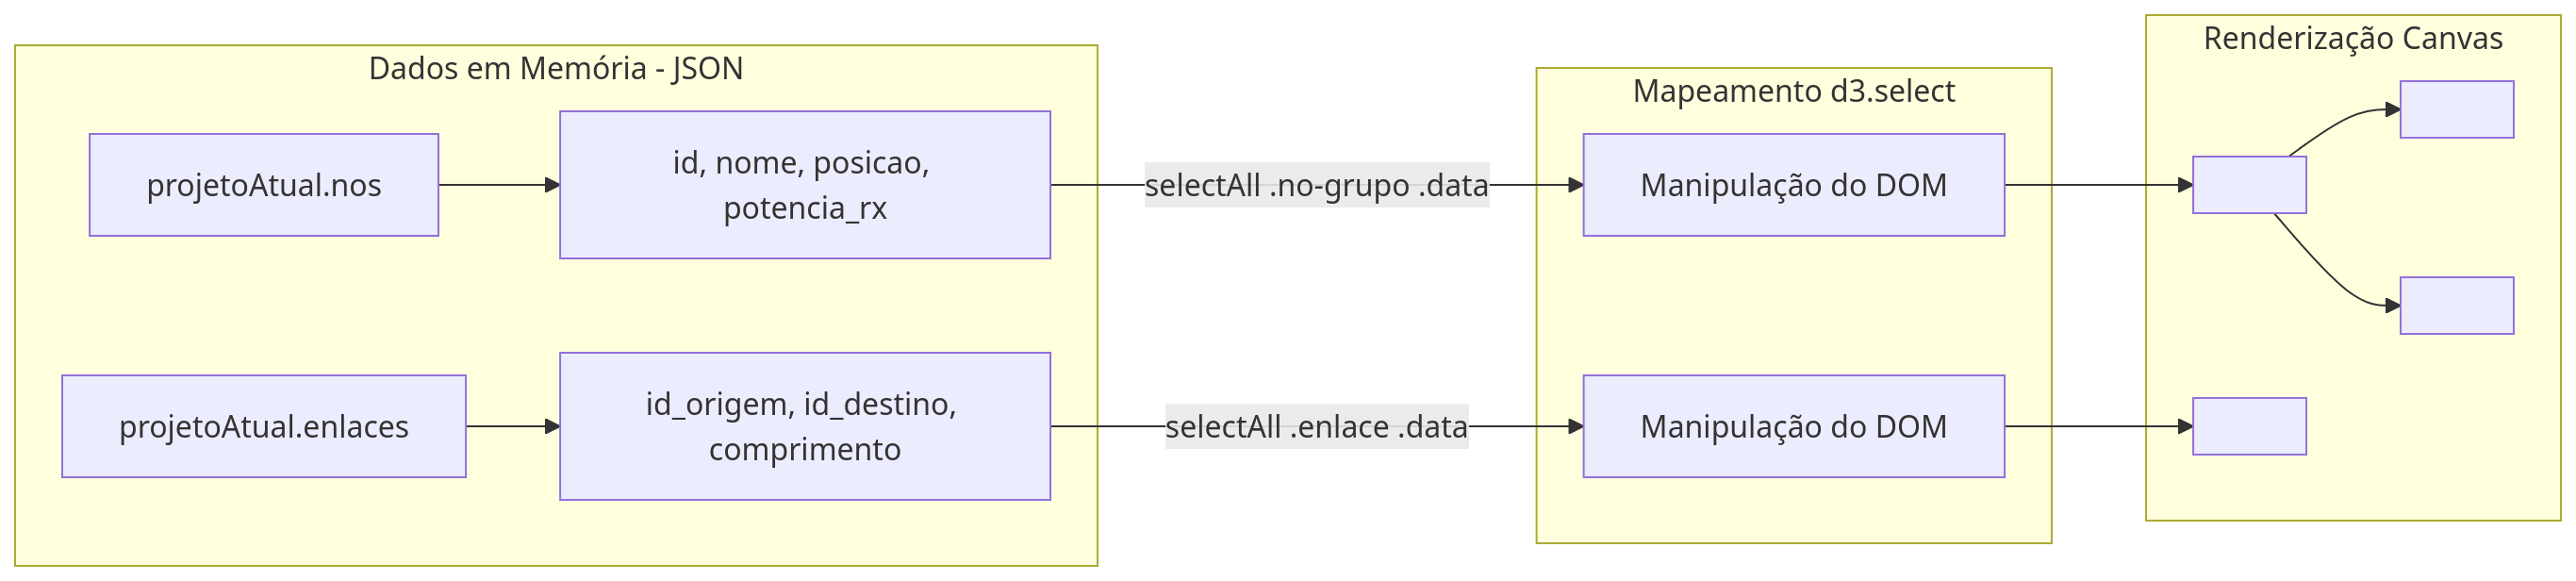
\includegraphics[width=0.85\textwidth]{images/estrutura_d3_canvas.png}
        \par\footnotesize Fonte: Elaboração própria com auxílio de IA.
    }
\end{figure}

O trecho de código a seguir demonstra o processo de renderização dos enlaces de fibra óptica:

\begin{verbatim}
// Desenho e atualização dos enlaces no contêiner SVG (<line>)
const enlaces = svg.selectAll(".enlace")
    .data(dadosProjeto.enlaces, d => d.id);

enlaces.enter()
    .append("line")
    .attr("class", "enlace")
    .merge(enlaces)
    .attr("x1", d => obterNoPorId(d.id_origem).posicao.x)
    .attr("y1", d => obterNoPorId(d.id_origem).posicao.y)
    .attr("x2", d => obterNoPorId(d.id_destino).posicao.x)
    .attr("y2", d => obterNoPorId(d.id_destino).posicao.y)
    .attr("stroke", "#0288d1")
    .attr("stroke-width", 2);

enlaces.exit().remove();
\end{verbatim}

O método \texttt{selectAll().data()} associa cada registro do \textit{array} de enlaces a uma tag \texttt{<line>} \gls{svg}. Durante a atualização, as coordenadas $(x_1, y_1)$ e $(x_2, y_2)$ são recalculadas com base nos nós de origem e destino.

Em seguida, o código cria os grupos de nós e adiciona o suporte ao arrasto (\textit{drag-and-drop}):

\begin{verbatim}
// Criação dos grupos de nós (<g>) com interatividade
const nos = svg.selectAll(".no-grupo")
    .data(dadosProjeto.nos, d => d.id);

const nosEnter = nos.enter()
    .append("g")
    .attr("class", "no-grupo")
    .call(d3.drag().on("drag", noArrastado));

nosEnter.append("circle")
    .attr("r", 18)
    .attr("fill", d => obterCorStatusSinal(d));

nosEnter.append("text")
    .attr("dy", 30)
    .attr("text-anchor", "middle")
    .text(d => `${d.nome} ${d.potencia_rx ? '(' + d.potencia_rx.toFixed(2) + ' dBm)' : ''}`);

nos.merge(nosEnter)
    .attr("transform", d => `translate(${d.posicao.x}, ${d.posicao.y})`);

nos.exit().remove();
\end{verbatim}

Cada nó é encapsulado em uma tag de grupo \texttt{<g>}, contendo um elemento \texttt{<circle>} (cuja cor reflete o status de sinal) e um elemento \texttt{<text>} (que exibe a potência calculada em dBm).

A movimentação dos nós na tela é tratada pela função \texttt{noArrastado}:

\begin{verbatim}
function noArrastado(event, d) {
    d.posicao.x = event.x;
    d.posicao.y = event.y;
    d3.select(this).attr("transform", `translate(${d.posicao.x}, ${d.posicao.y})`);
    atualizarLinhasEnlaces();
}
\end{verbatim}

\subsection{Comunicação Assíncrona e Reatividade}

A reatividade do sistema ocorre pelo envio assíncrono do estado do grafo para a \gls{api} FastAPI através do método \texttt{fetch}:

\begin{verbatim}
async function calcularOrcamentoOptico() {
    try {
        const response = await fetch('/api/calculo', {
            method: 'POST',
            headers: { 'Content-Type': 'application/json' },
            body: JSON.stringify(projetoAtual)
        });

        if (!response.ok) {
            throw new Error(`Erro na requisição: ${response.statusText}`);
        }

        const resposta = await response.json();

        if (resposta.status === 'sucesso') {
            atualizarValoresPotencia(resposta.dados.nos);
            atualizarGrafo(projetoAtual);
        }
    } catch (erro) {
        console.error("Erro ao sincronizar orçamento óptico:", erro);
    }
}
\end{verbatim}

Sempre que o usuário move um nó ou altera uma propriedade no painel lateral, esta função transmite o \gls{json} do projeto e aplica o resultado retornado sem a necessidade de recarregar a página web.